\section{Introduction}

%% adapt introduction to make it more friendly, but not too verbose.
%%
%% write the outline more specific towards the main idea of the thesis,
%% namely fuzzing rxe, different approaches, evaluation.
%%
%% Maksyms input:  I would suggest to prioritise the sections where you have more data
%% given that you try diff approaches, sllight different structure of section,
%% instead of normal design, impl and evauluation
%% user level fuzzing, network level fuzzing, evaluation
%%
In the setting of High Performance Computing and cloud, technologies like InfiniBand, which enable Remote Direct Memory Access
(RDMA) have been gaining considerable importance in the last decades.

As the combination IP/Ethernet is an ubiquitous technology, the need for a technology similar
to the one used by InfiniBand networks which allows
RDMA without having to resort to specialized hardware arised. RDMA over Converged Ethernet (RoCE) is an modification
to the InfiniBand stack, which replaces the link and physical layers for those of Ethernet,
allowing to use regular switches to provide InfiniBand services. Since  RoCE traffic does not carry an IP header,
it cannot be routed across the boundaries of Ethernet networks using regular IP routers\cite{rocev2}.

The RoCEv2 specification is an extension of the former, it allows routers to transport
IB packets contained within a UDP datagram over the IP protocol. But Nevertheless, RDMA operations still require RoCE adapter
cards as to take the involvement of the OS out of the picture.

An open source software implementation of the RDMA transport, called SoftRoCE, has been part of the mainline tree of
the linux kernel since late 2016. SoftRoCE is implemented as a device driver and it provides a complete RDMA
stack implementation over any regular NIC\cite{softroce}.

More importantly, SoftRoCE enables interoperation between a server equipped with a RoCE adapter card, and a server running on
commodity hardware. The fact that any hardware and even VMs can be part of an RDMA architecture, bridges an important gap in the RDMA ecosystem.

\begin{figure}[h]
  \centering
  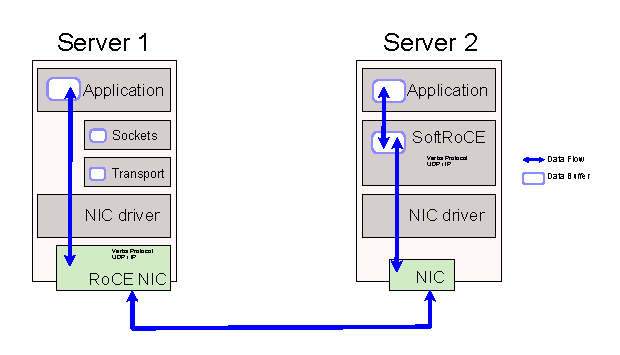
\includegraphics[]{softrocepretty}
  \caption[softroce]{SoftRoCE allows RDMA interaction with RoCE devices\footnotemark}
\end{figure}

\footnotetext{adapted from \url{ https://www.roceinitiative.org/wp-content/uploads/2016/11/SoftRoCE_Paper_FINAL.pdf }}

Given the relevance and usefulness of SoftRoCE, as well as the monolithic nature of the linux kernel,
it is a major concern for SoftRoCE it to be safe and reliable.
Using a software testing technique which has been gaining popularity recently due to its efficiency in
discovering bugs, namely fuzzing, this work aims to explore and describe ways to identify the attack surface
of this particular device driver and the API it exposes.

For very complex systems like the linux kernel, with over thirteen million lines of code, merely auditing the
source code for vulnerability discovery (by means of e.g. code reviews or static analysis tools) is not enough.
Fuzzing has been a succesful tool in unveiling a wide variety of vulnerabilities in open source projects like chromium,
firefox and the linux kernel (TODO add citations).

Software is nowadays designed by programmers with a well defined scenario in mind. Most of the time, software tests
are routinely written in a way so that the expected behaviour of a program still holds, given expected input, i.e. the input
the program was designed for.

Fuzzing is a testing technique does not require any kind of knowledge from the target program (also commonly addressed as system under test),
as the basic idea it bases upon is to throw random input into the application until it breaks or something unintended happens. Under
this basic idea of what defines fuzzing, we will evaluate different approaches and assert their effectiveness or usefulness
at putting SoftRoCE under stress.
